\documentclass[12pt]{article}

\usepackage{algorithm} %pseudo-code
\usepackage{algpseudocode}
\usepackage{amsmath,amsthm,amssymb}
\usepackage{graphicx}
\usepackage{float}
\usepackage{amsmath, amssymb, amscd}
\usepackage{alltt}
\usepackage{textcomp}
\usepackage{gensymb}
\usepackage{multicol}
\usepackage{tabularx}

\newcommand{\N}{\mathcal{N}}
\newcommand{\Z}{\mathbb{Z}}
\newcommand{\R}{\mathbb{R}}
\newcommand{\bigo}{\mathcal{O}}
\newcommand{\G}{\mathcal{G}}
\newcommand{\V}{\mathcal{V}}
\newcommand{\E}{\mathcal{E}}
\newcommand{\K}{\mathcal{K}}
\newcommand{\T}{^\intercal}

\newcommand{\sups}[1]{\ensuremath{^{\textrm{#1}}}}
\newcommand{\subs}[1]{\ensuremath{_{\textrm{#1}}}}

\newcommand{\specialcell}[2][c]
{
  \begin{tabular}[#1]{@{}c@{}}#2\end{tabular}
}

\makeatletter
\newsavebox{\mybox}\newsavebox{\mysim}
\newcommand{\distras}[1]
{
  \savebox{\mybox}{\hbox{\kern3pt$\scriptstyle#1$\kern3pt}}%
  \savebox{\mysim}{\hbox{$\sim$}}%
  \mathbin{\overset{#1}{\kern\z@\resizebox{\wd\mybox}{\ht\mysim}{$\sim$}}}%
}
\makeatother
\makeatletter
\renewcommand*\env@matrix[1][c]{\hskip -\arraycolsep
  \let\@ifnextchar\new@ifnextchar
  \array{*\c@MaxMatrixCols #1}}
\makeatother
%===============================================================================
% code highlighting :
\usepackage{listings}

% define custom colors :
\usepackage{color}
\definecolor{bg}{rgb}{0.96,0.96,0.85}
\definecolor{deepblue}{rgb}{0,0,0.5}
\definecolor{deepred}{rgb}{0.6,0,0}
\definecolor{deepgreen}{rgb}{0,0.5,0}

\usepackage{xcolor}
\renewcommand{\lstlistlistingname}{Code Listings}
\renewcommand{\lstlistingname}{Code Listing}
\definecolor{gray}{gray}{0.5}
\colorlet{commentcolour}{green!50!black}

\colorlet{stringcolour}{red!60!black}
\colorlet{keywordcolour}{magenta!90!black}
\colorlet{exceptioncolour}{yellow!50!red}
\colorlet{commandcolour}{blue!60!black}
\colorlet{numpycolour}{blue!60!green}
\colorlet{literatecolour}{magenta!90!black}
\colorlet{promptcolour}{green!50!black}
\colorlet{specmethodcolour}{violet}
\colorlet{indendifiercolour}{green!70!white}

\newcommand{\framemargin}{5ex}

\newcommand{\literatecolour}{\textcolor{literatecolour}}

\newcommand\pythonstyle{\lstset{
%keepspaces=true,
language=python,
showtabs=true,
tab=,
tabsize=2,
basicstyle=\ttfamily\scriptsize,%\setstretch{.5},
stringstyle=\color{stringcolour},
showstringspaces=false,
alsoletter={1234567890},
otherkeywords={\ , \}, \{, \%, \&, \|},
keywordstyle=\color{keywordcolour}\bfseries,
emph={and,break,class,continue,def,yield,del,elif ,else,%
except,exec,finally,for,from,global,if,import,in,%
lambda,not,or,pass,print,raise,return,try,while,assert},
emphstyle=\color{blue}\bfseries,
emph={[2]True, False, None},
emphstyle=[2]\color{keywordcolour},
emph={[3]object,type,isinstance,copy,deepcopy,zip,enumerate,reversed,list,len,dict,tuple,xrange,append,execfile,real,imag,reduce,str,repr},
emphstyle=[3]\color{commandcolour},
emph={Exception,NameError,IndexError,SyntaxError,TypeError,ValueError,OverflowError,ZeroDivisionError},
emphstyle=\color{exceptioncolour}\bfseries,
%upquote=true,
morestring=[s]{"""}{"""},
morestring=[s]{'''}{'''},
commentstyle=\color{commentcolour}\slshape,
%emph={[4]1, 2, 3, 4, 5, 6, 7, 8, 9, 0},
emph={[4]ode, fsolve, sqrt, exp, sin, cos, arccos, pi,  array, norm, solve, dot, arange, , isscalar, max, sum, flatten, shape, reshape, find, any, all, abs, linspace, legend, quad, polyval,polyfit, hstack, concatenate,vstack,column_stack,empty,zeros,ones,rand,vander,grid,pcolor,eig,eigs,eigvals,svd,qr,tan,det,logspace,roll,min,mean,cumsum,cumprod,diff,vectorize,lstsq,cla,eye,xlabel,ylabel,squeeze,plot,median,std,hist},
emphstyle=[4]\color{numpycolour},
emph={[5]__init__,__add__,__mul__,__div__,__sub__,__call__,__getitem__,__setitem__,__eq__,__ne__,__nonzero__,__rmul__,__radd__,__repr__,__str__,__get__,__truediv__,__pow__,__name__,__future__,__all__},
emphstyle=[5]\color{specmethodcolour},
emph={[6]assert,range,yield},
emphstyle=[6]\color{keywordcolour}\bfseries,
% emph={[7]self},
% emphstyle=[7]\bfseries,
literate=*%
{:}{{\literatecolour:}}{1}%
{=}{{\literatecolour=}}{1}%
{-}{{\literatecolour-}}{1}%
{+}{{\literatecolour+}}{1}%
{*}{{\literatecolour*}}{1}%
{/}{{\literatecolour/}}{1}%
{!}{{\literatecolour!}}{1}%
%{(}{{\literatecolour(}}{1}%
%{)}{{\literatecolour)}}{1}%
{[}{{\literatecolour[}}{1}%
{]}{{\literatecolour]}}{1}%
{<}{{\literatecolour<}}{1}%
{>}{{\literatecolour>}}{1}%
{>>>}{{\textcolor{promptcolour}{>>>}}}{1}%
,%
breaklines=true,
breakatwhitespace= true,
%xleftmargin=\framemargin,
%xrightmargin=\framemargin,
aboveskip=1ex,
frame=trbl,
%frameround=tttt,
rulecolor=\color{black!40},
%framexleftmargin=\framemargin,
%framextopmargin=.1ex,
%framexbottommargin=.1ex,
%framexrightmargin=\framemargin,
%framexleftmargin=1mm, framextopmargin=1mm, frame=shadowbox, rulesepcolor=\color{blue},#1
%frame=tb,
backgroundcolor=\color{yellow!10}
}}

% Python environment
\lstnewenvironment{python}[1][]
{
  \pythonstyle
  \lstset{#1}
}
{}

% Python for external files
\newcommand\pythonexternal[1]
{{
  \pythonstyle
  \lstinputlisting{#1}
}}

% Python for inline
\newcommand\pythoninline[1]{{\pythonstyle\lstinline!#1!}}

% end code highlighting
%===============================================================================

\usepackage{tabularx}
\DeclareMathOperator*{\argmax}{arg\,max}

\begin{document}
\small

\title{Space Simulator - Project 05}
\author{Evan Cummings and Joshua Bartz\\
CSCI 576 - Human Computer Interaction}

\maketitle

\section{Test plan}

\subsection{Purpose}

We shall perform 4-5 tests with users on the system in order to better understand any learning, operation, or interpretive challenges presented by the simulator.

\subsection{Objectives}

The objectives of the test are to analyze the effectiveness of the navigation display, control of the craft, and user's ability to correct mistakes.

\subsection{User profile}

Users should have a familiarity with video games, preferably flight simulators.  The level of difficulty demands patience and interest in the subject matter.  Therefore, we will choose mature pilots who have a genuine interest in the system. Some kind of background in mathematics and/or physics will be very helpful.

\subsection{Environment}

The test environment should be comfortable to the user and free of outside distractions.  In order to analyze the results at a later time, the sessions will be video and audio recorded via a single camera placed over the user's shoulder and aimed at the screen.  A computer with a decent video card and processor will be required in order to play the game with optimal performance.

\subsection{Roles of test givers}

Evan will be the test administrator and handle the camera while Josh will read the test script and note questions.  Both Evan and Josh will take notes and ask post-test interview questions.

\subsection{Evaluation}

During the test sessions, we will note any frustrations of the users in controlling the craft.  It will be important to distinguish between frustrations with the controls and frustrations with the physics of space.  Because the game is designed as a space simulator, users may expect to continue flying forward in the direction they are facing, but in space this is not the case.

We will measure the amount of time or number of attempts to complete a task, as well and the accompanying emotional response of the participants.

\section{Test materials}

\subsection{Test script}

Hello, and welcome to Space Simulator, a new and innovative space-flight simulator.  We'd like to take this opportunity to thank you for volunteering your time to help us test this new and exciting adventure.  I will be reading from this script to ensure consistency between all of our participants.

Now a little about Space Simulator.  Space Simulator is a simulation of what it would be like to actually pilot a craft in outer space, using realistic physics.  Please note that Space Simulator is still in its development stage and that it may break down under certain circumstances.  If that does happen, we will restart the program. 
  
Understand that this exercise is to test the product and its usability, and is in no way a test of your abilities.  If at any time you feel uncomfortable, please inform us and we will terminate the exercise immediately. (We will be recording this exercise so that we can gather as much information as possible from this session).
   
Your opinion and ideas are important to us.  Whenever possible, please speak your thoughts freely.  Do not be concerned about offending us.  If you forget to think aloud, I'll remind you to keep talking. 
    
As you’re working through Space Simulator, I won’t be able to provide help or answer questions.  This is because we want to create the most realistic situation possible.  Even though I won't be able to answer your questions during the exercise, please ask them. We'll note your questions and answer them at the end of the exercise. 
     
Do you have any questions? 

\subsection{Checklist}

\noindent
\textbf{Pre-study:}
\begin{itemize}
  \item Boot up the computer with packages pre-installed and simulation tested in advance.
  \item Navigate to the folder containing the program.
  \item type in the terminal the command to execute the simulation.
\end{itemize}

\noindent
\textbf{Study:}
\begin{itemize}
  \item Read the test script to the participant(s).
  \item Begin video recording.
  \item Ask the participant(s) if they have any questions.
  \item Have the user execute the program and begin the testing.
\end{itemize}

\noindent
\textbf{Post-study:}
\begin{itemize}
  \item Ask users not to discuss experiment with others.
  \item Perform post-test interview.
  \item Have the users fill out the post-test questionnaire.
\end{itemize}

\subsection{Data capture form}

See accompanying attachment.

\subsection{Task list}

\begin{enumerate}

  \item \textbf{Control familiarization!}  A comprehensive walk-through of all of the directional controls used to pilot the ship. 

  Tasks:
  \begin{itemize}
    \item Launch the game by typing ``\texttt{python spaceSimulator.py}''
    \item Pause the game
    \item Review controls
    \item Resume game
    \item Accelerate the ship forward until the velocity vector reads at least 15.0
    \item Bring the ship to a stop
    \item Accelerate in the left direction until the velocity vector reads at least 15.0
    \item Bring the ship to a stop
    \item Exit the game
  \end{itemize}
  
  \item \textbf{Rotation  familiarization!}  A comprehensive walk-through of all of the directional controls used to pilot the ship. 

  Tasks:
  \begin{itemize}
    \item Launch the game by typing ``\texttt{python spaceSimulator.py}''
    \item Pause the game
    \item Review controls
    \item Resume game
    \item Pitch the ship up until the angular velocity vector reads at least 1.0
    \item After the ship rotates 360 degrees, stop the ship.
    \item Yaw the craft until the angular velocity vector reads at least 1.0
    \item After the ship rotates 360 degrees, stop the ship.
    \item Exit the game
  \end{itemize}
  
  \item \textbf{Collision correction.}  You will begin a new game, then attempt to fly into one of the ``asteroids.''  After the collision, your ship will behave erratically, and you will need to fix it.
  
  Tasks:
  \begin{itemize}
    \item Launch the game by typing ``\texttt{python spaceSimulator.py}''
    \item Locate an asteroid/planet by any means
    \item Pilot the ship into a collision course with the asteroid/planet
    \item Collide with the asteroid/planet
    \item Take note of the force vectors acting on the craft
    \item One direction at a time, bring the ship to a complete stop
    \item Exit the game
  \end{itemize}
  
  \item \textbf{Experiment!}  Time for some free-flying.  Taking the controls you have learned, fly for 3-5 minutes. 
  
  Tasks:
  \begin{itemize}
    \item Launch the game by typing ``\texttt{python spaceSimulator.py}''
    \item For 3-5 minutes, practice using the controls
    \item Attempt near-misses with the asteroids and planet
    \item See how fast you can move the ship in multiple directions without losing control
    \item See how long you can maintain orbit of the planet
  \end{itemize}

\end{enumerate}

\subsection{Post-test questionnaire}

After completing the test we gave the participants this questionnaire:

\vspace{10mm}
\noindent Please circle your answer or write a response in the space provided.

\vspace{5mm}
\noindent\textbf{Name:}

\vspace{5mm}
\noindent\textbf{Please indicate your age range:}
\begin{enumerate}
  \item 18-25
  \item 26-30
  \item 31-35
  \item 36 and up
\end{enumerate}

\vspace{5mm}
\noindent\textbf{How many hours per week do you play video games?}
\begin{enumerate}
  \item 0
  \item 1-3
  \item 4-6
  \item 6-9
  \item 10+
\end{enumerate}

\vspace{5mm}
\noindent\textbf{What is your physics background?}
\begin{enumerate}
  \item No background
  \item High school
  \item 1-2 classes in college
  \item 3+ classes in college
  \item Other
\end{enumerate}
If other, please explain:

\vspace{5mm}
\noindent\textbf{Have you ever played any kind of flight simulator before?} Y N

\vspace{5mm}
\noindent\textbf{If yes, have you ever played a spaceflight simulator before?} Y N

\vspace{5mm}
\noindent\textbf{When playing PC games, what kind of controls do you prefer?} Y N
\begin{enumerate}
  \item Mouse/keyboard
  \item Gamepad
  \item Joystick
  \item Other
  \item I don’t play PC games
\end{enumerate}
If other, please explain:

\vspace{5mm}
\noindent\textbf{Have you ever taken a course in Linear Algebra?} Y N

\vspace{5mm}
\noindent\textbf{On a scale of 1 to 5, one being not at all interested, 5 being very interested, how interested are you in spaceflight?} Y N

\vspace{5mm}
\noindent\textbf{On a scale of 1 to 5, one being not at all important, 5 being very important, how important are graphics to you when you are playing a game?} Y N

\subsection{Post-test interview}

\vspace{5mm}
\noindent\textbf{How did you like the controls?}

\vspace{5mm}
\noindent\textbf{What would you like changed or added?}

\vspace{5mm}
\noindent\textbf{Did you find the on-screen vectors to be providing clear and useful information?}

\vspace{5mm}
\noindent\textbf{Did you find the simulation, overall, to be realistic?}

\vspace{5mm}
\noindent\textbf{What, if anything, gave you problems that hasn't already been discussed?}

\section{Analysis}

These tests highlighted many problems already known to us, and a few that were not.  All participants found the game challenging, with one even asking to stop the test out of frustration.  However, we noticed that the pair of participants seemed to enjoy the game a bit more; we believe this is because they could communicate ideas to each other and felt a bit less exposed.  All the participants who worked alone except one became embarrassed that they could not pilot the craft correctly, to the point of frustration.  As a result, these players did not perform as well.

\subsection{Video recording screenshots}

\begin{figure}[H]
  \centering
  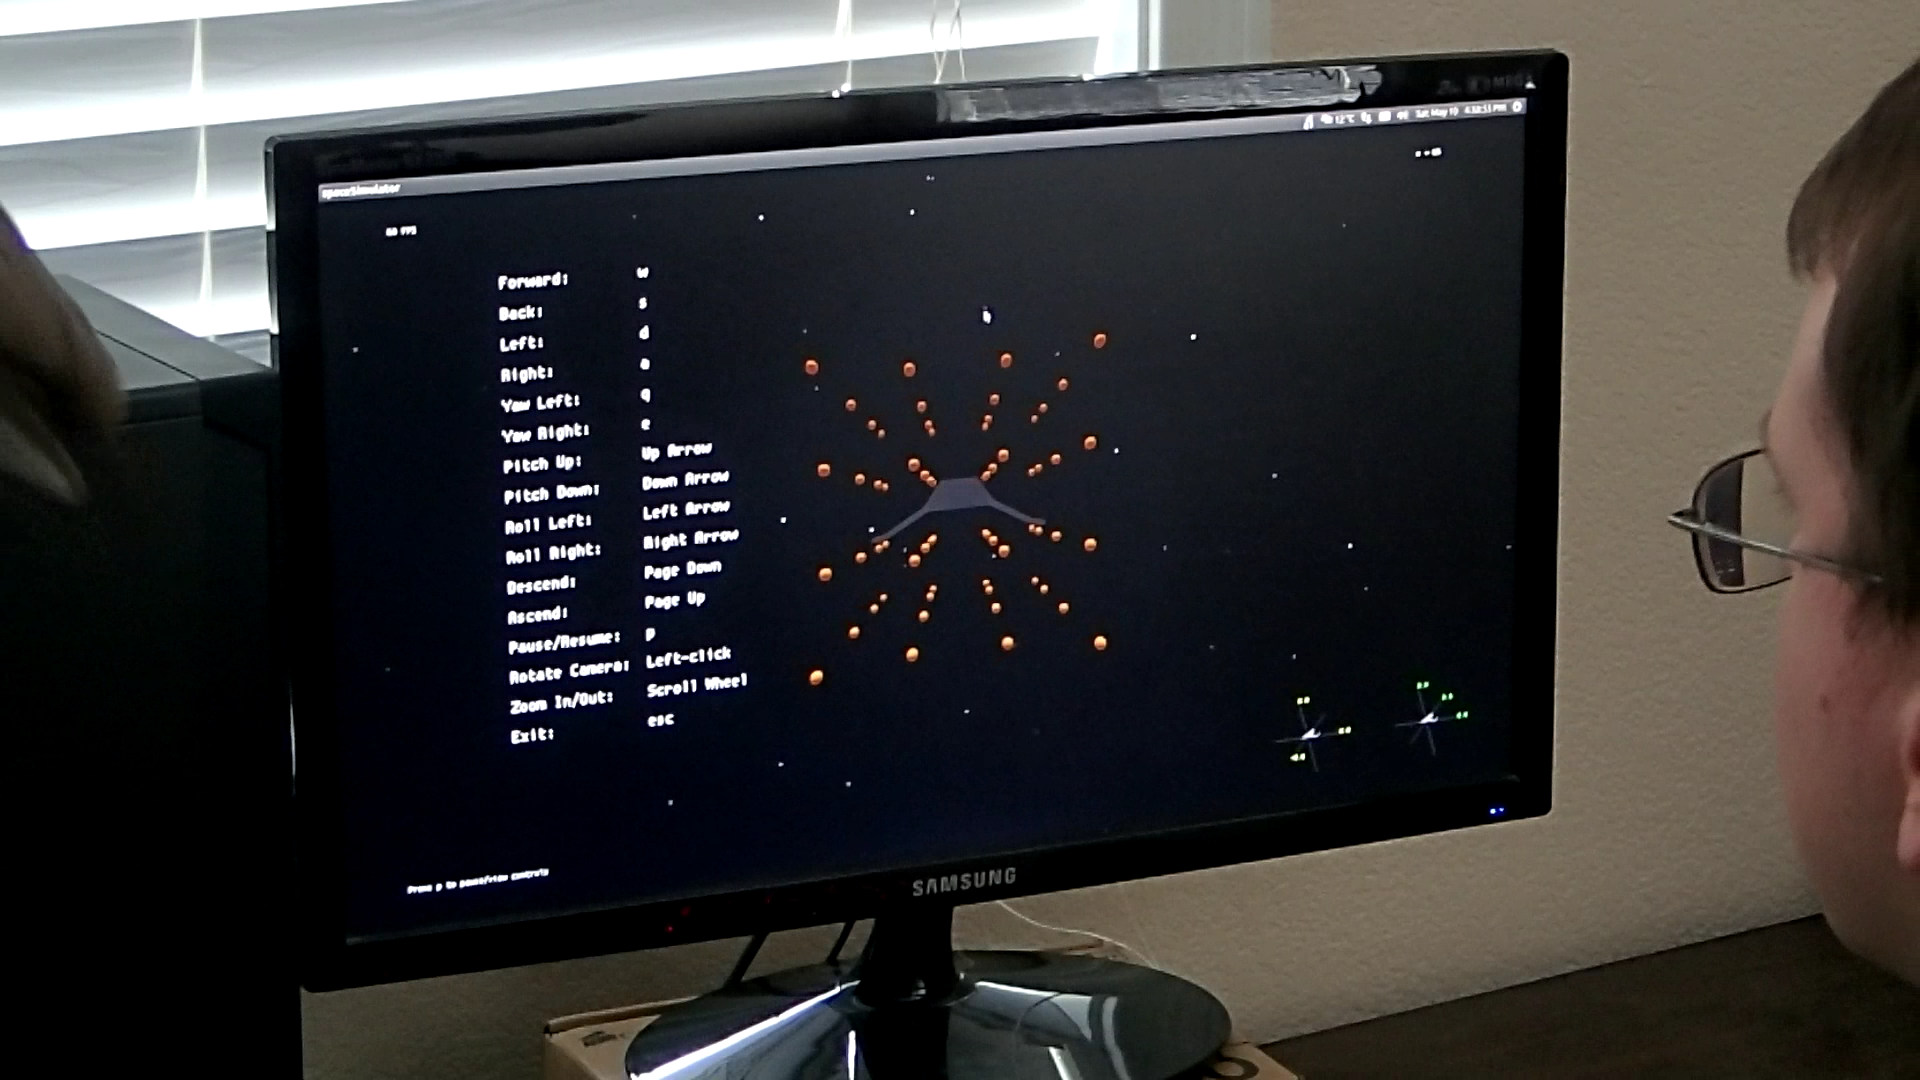
\includegraphics[width=1.0\textwidth]{images/ss1.jpg}
  \caption{Here we have a test-subject reviewing the controls, a frequent occurrence.}
\end{figure}

\begin{figure}[H]
  \centering
  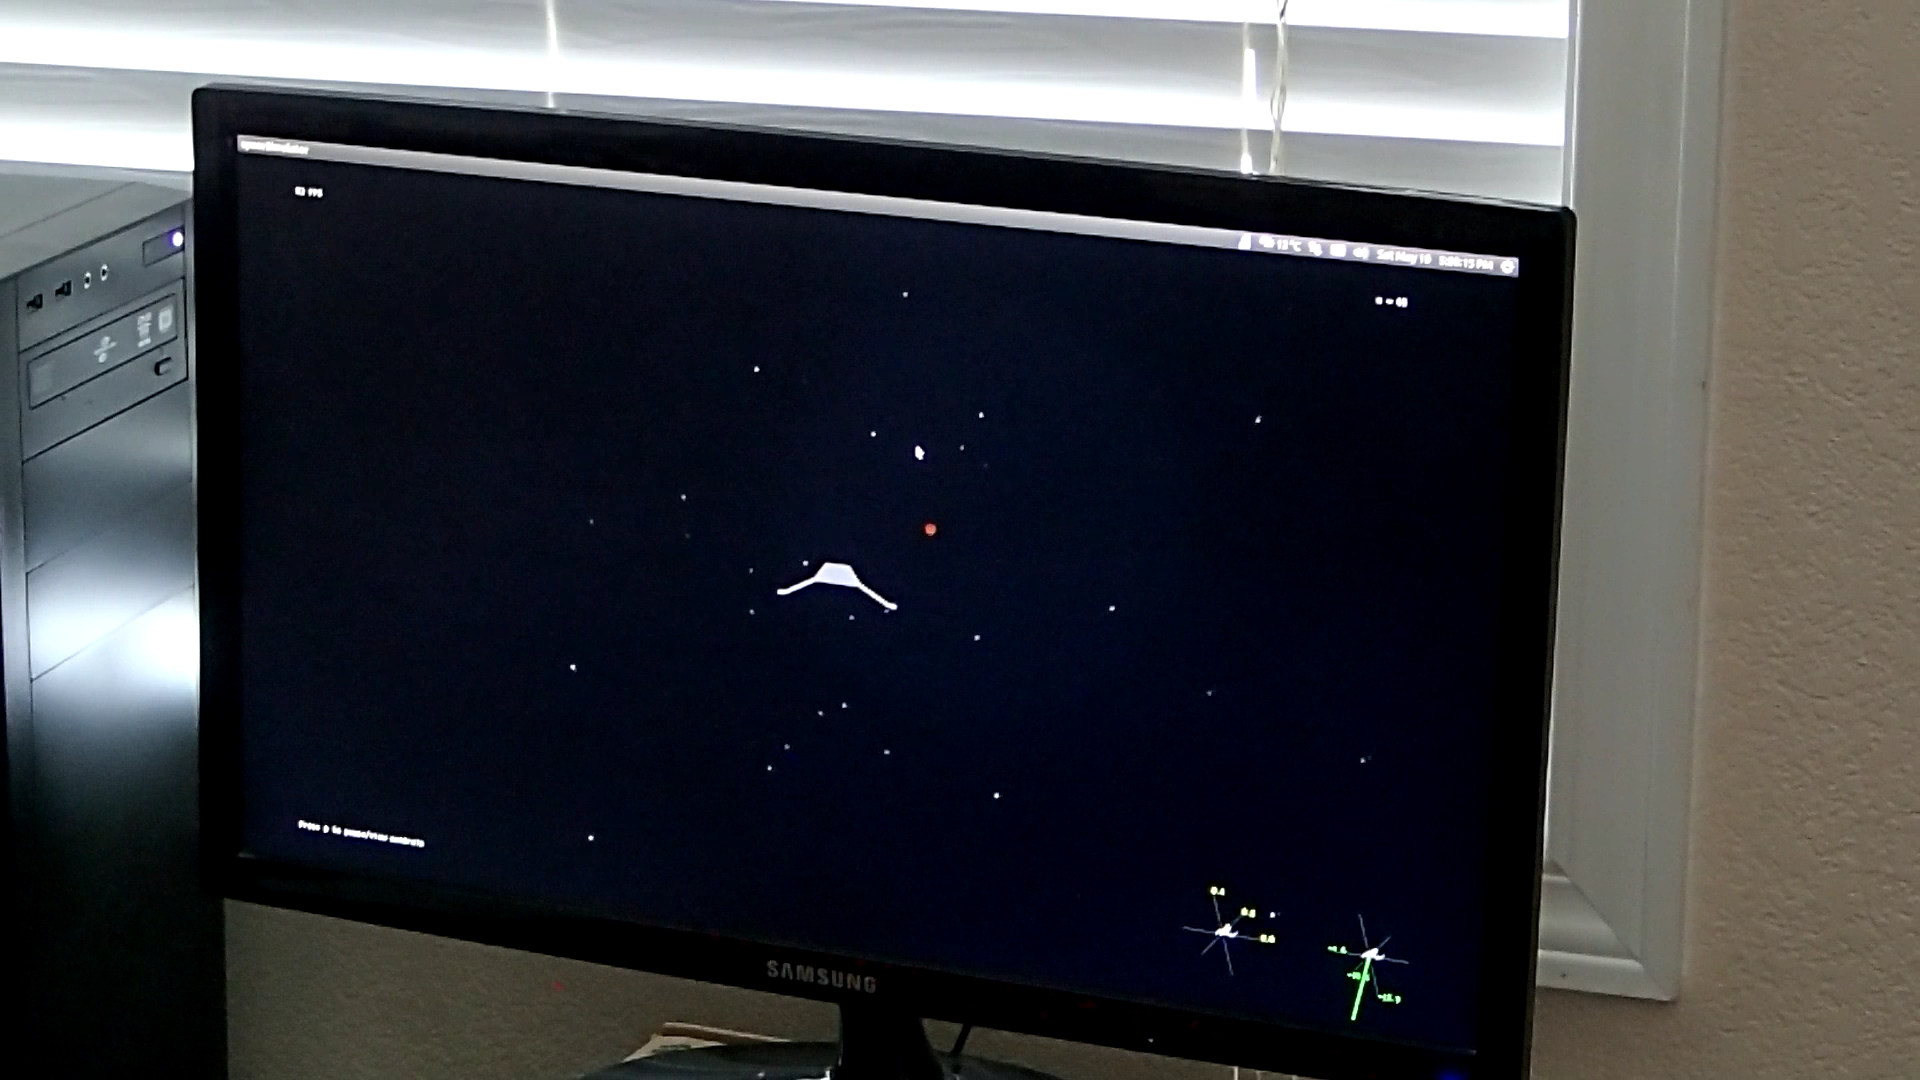
\includegraphics[width=1.0\textwidth]{images/ss2.jpg}
  \caption{A user attempting to reach a planet, with great difficulty.  Gameplay for the initial test sessions was to fast, making the craft difficult to control.}
\end{figure}

\begin{figure}[H]
  \centering
  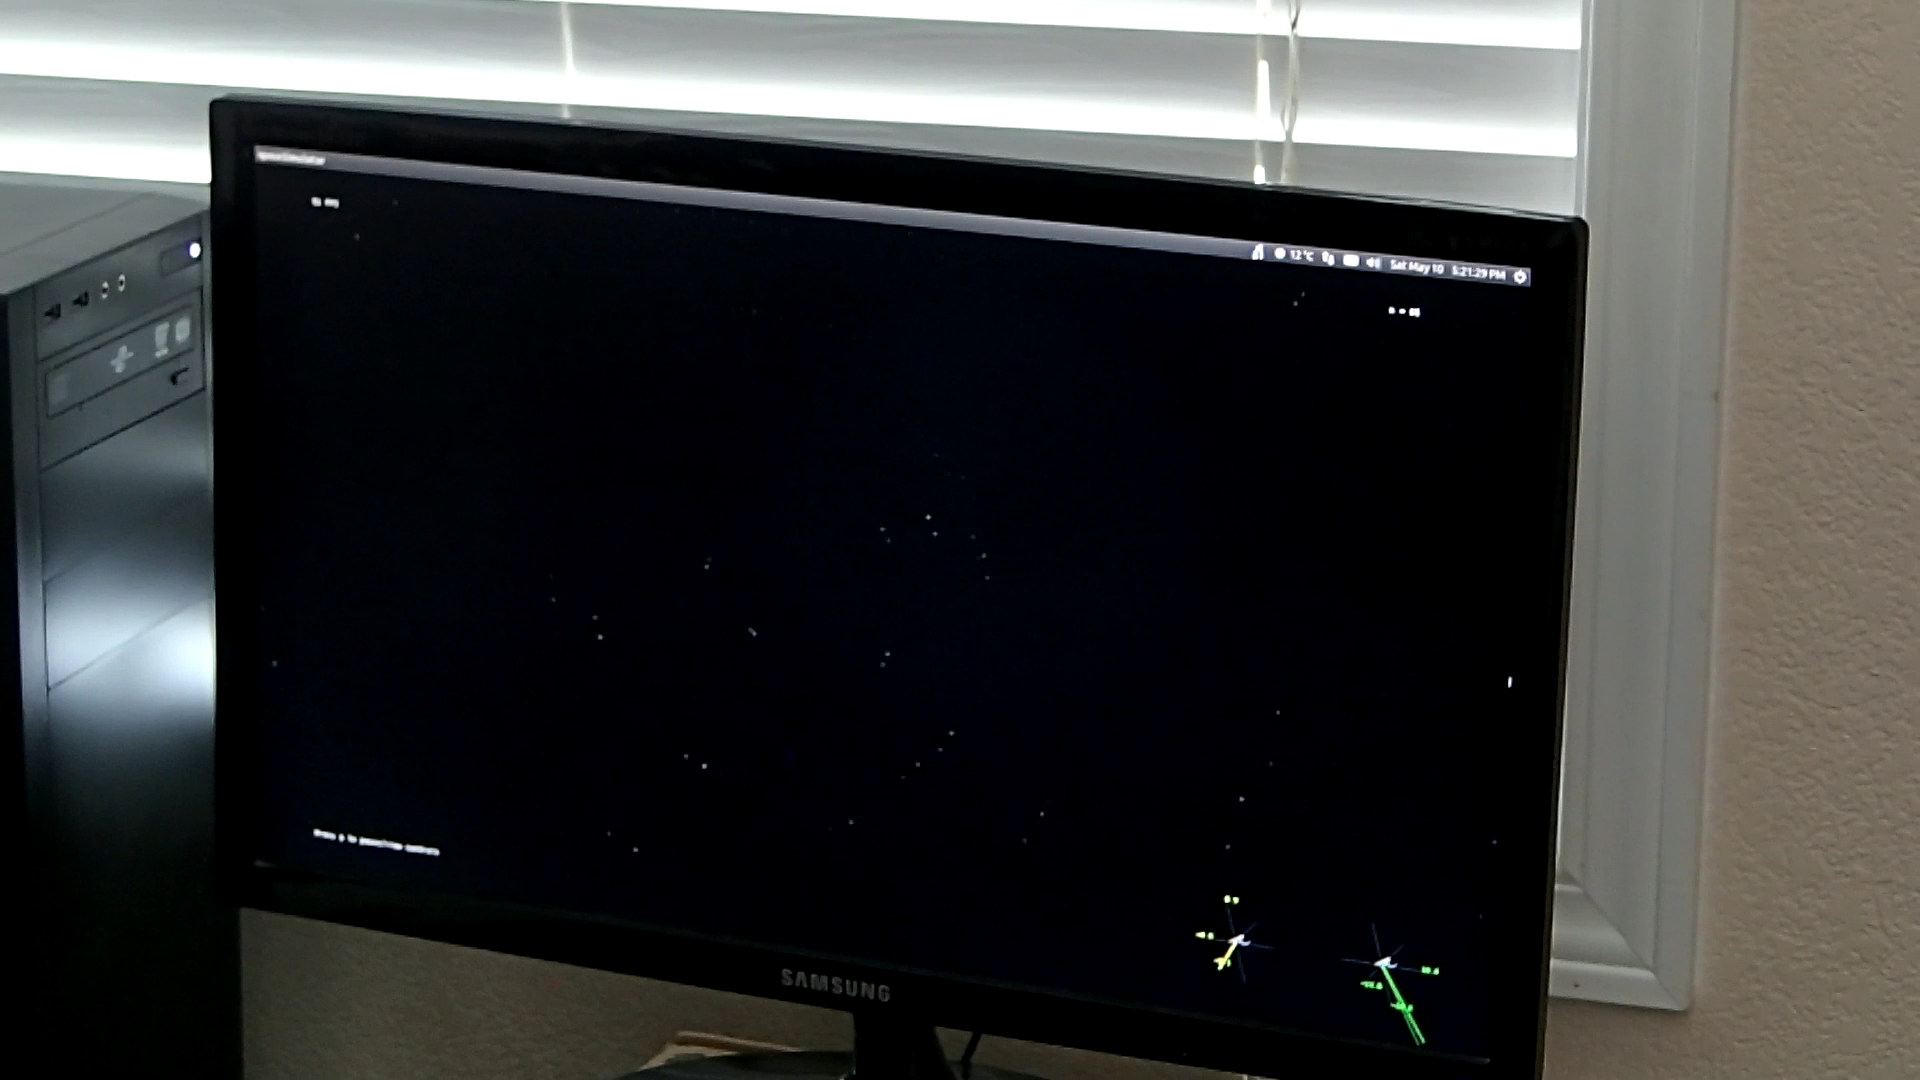
\includegraphics[width=1.0\textwidth]{images/ss3.jpg}
  \caption{Lost in space, rotating in circles without the ability to stop.  The game is difficult.}
\end{figure}

\begin{figure}[H]
  \centering
  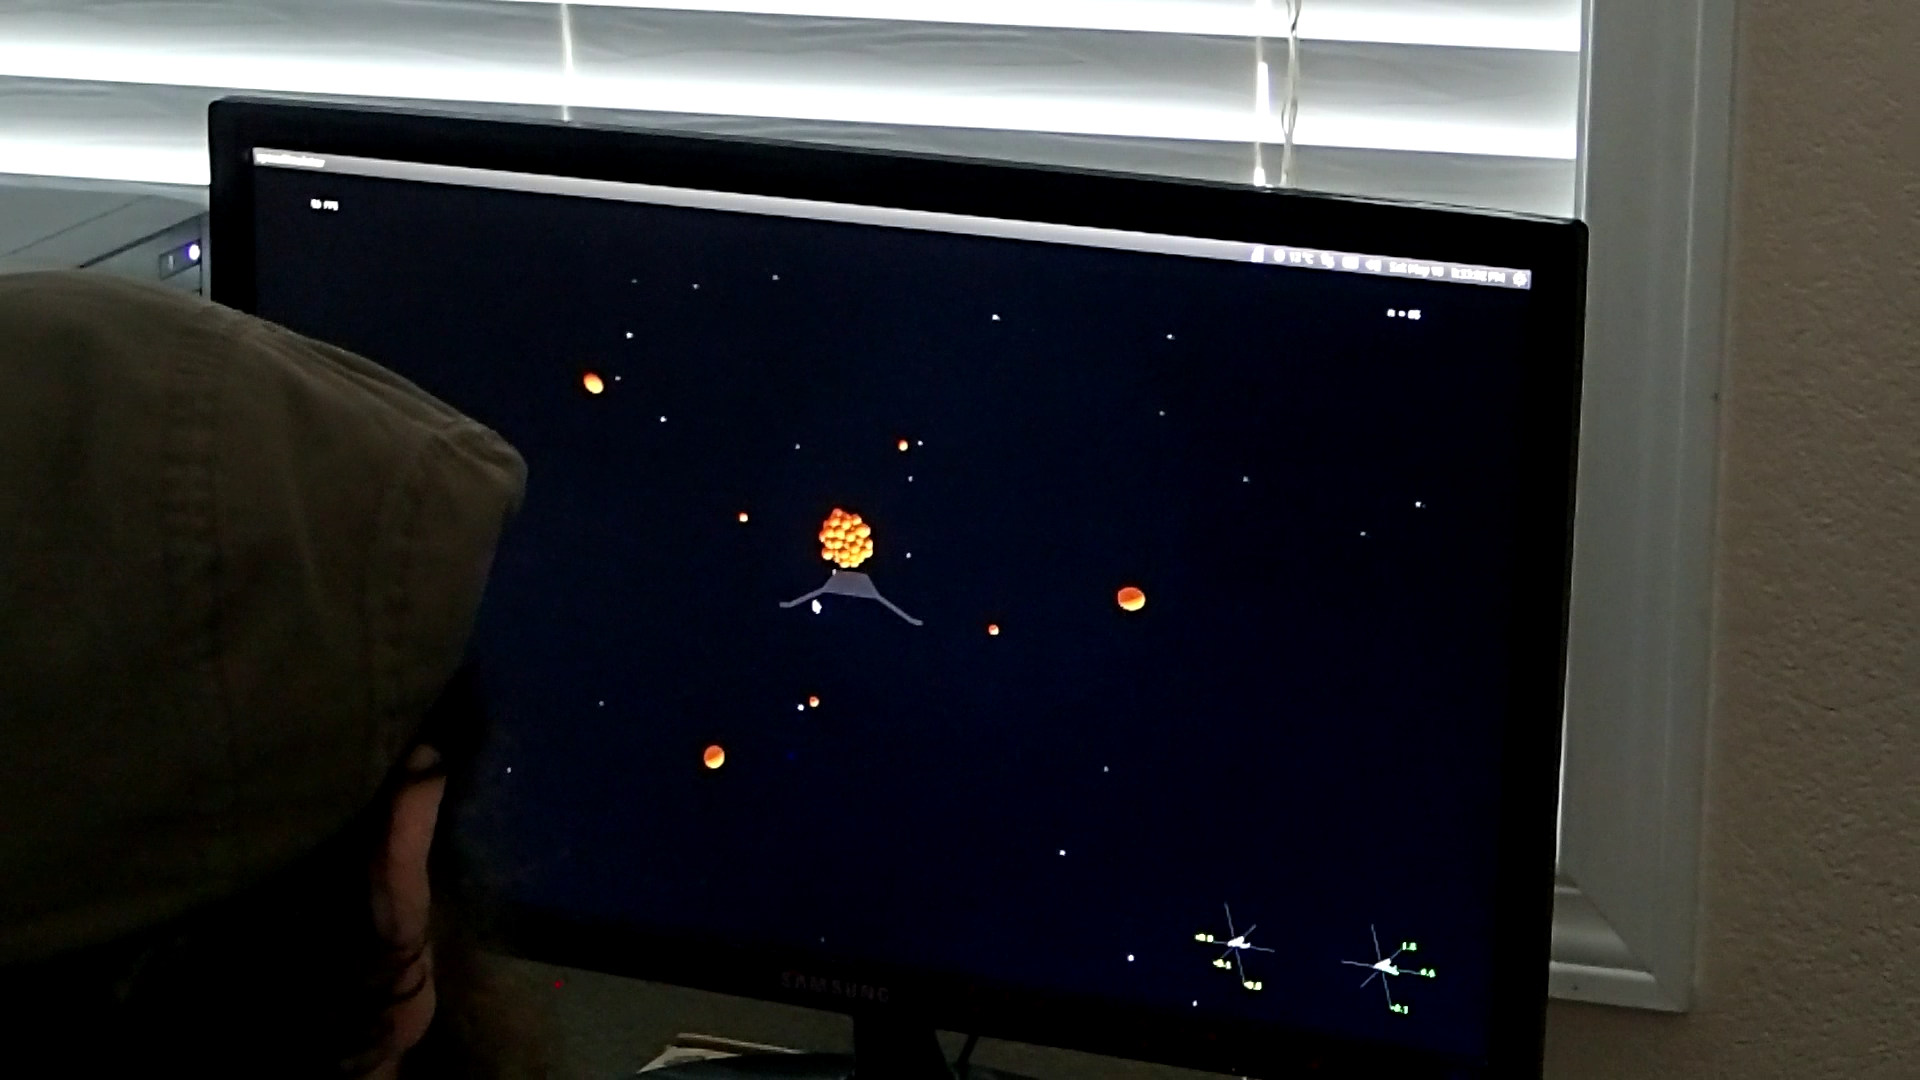
\includegraphics[width=1.0\textwidth]{images/ss4.jpg}
  \caption{Here a user has successfully remained close to the planet, for the time being.}
\end{figure}

\begin{figure}[H]
  \centering
  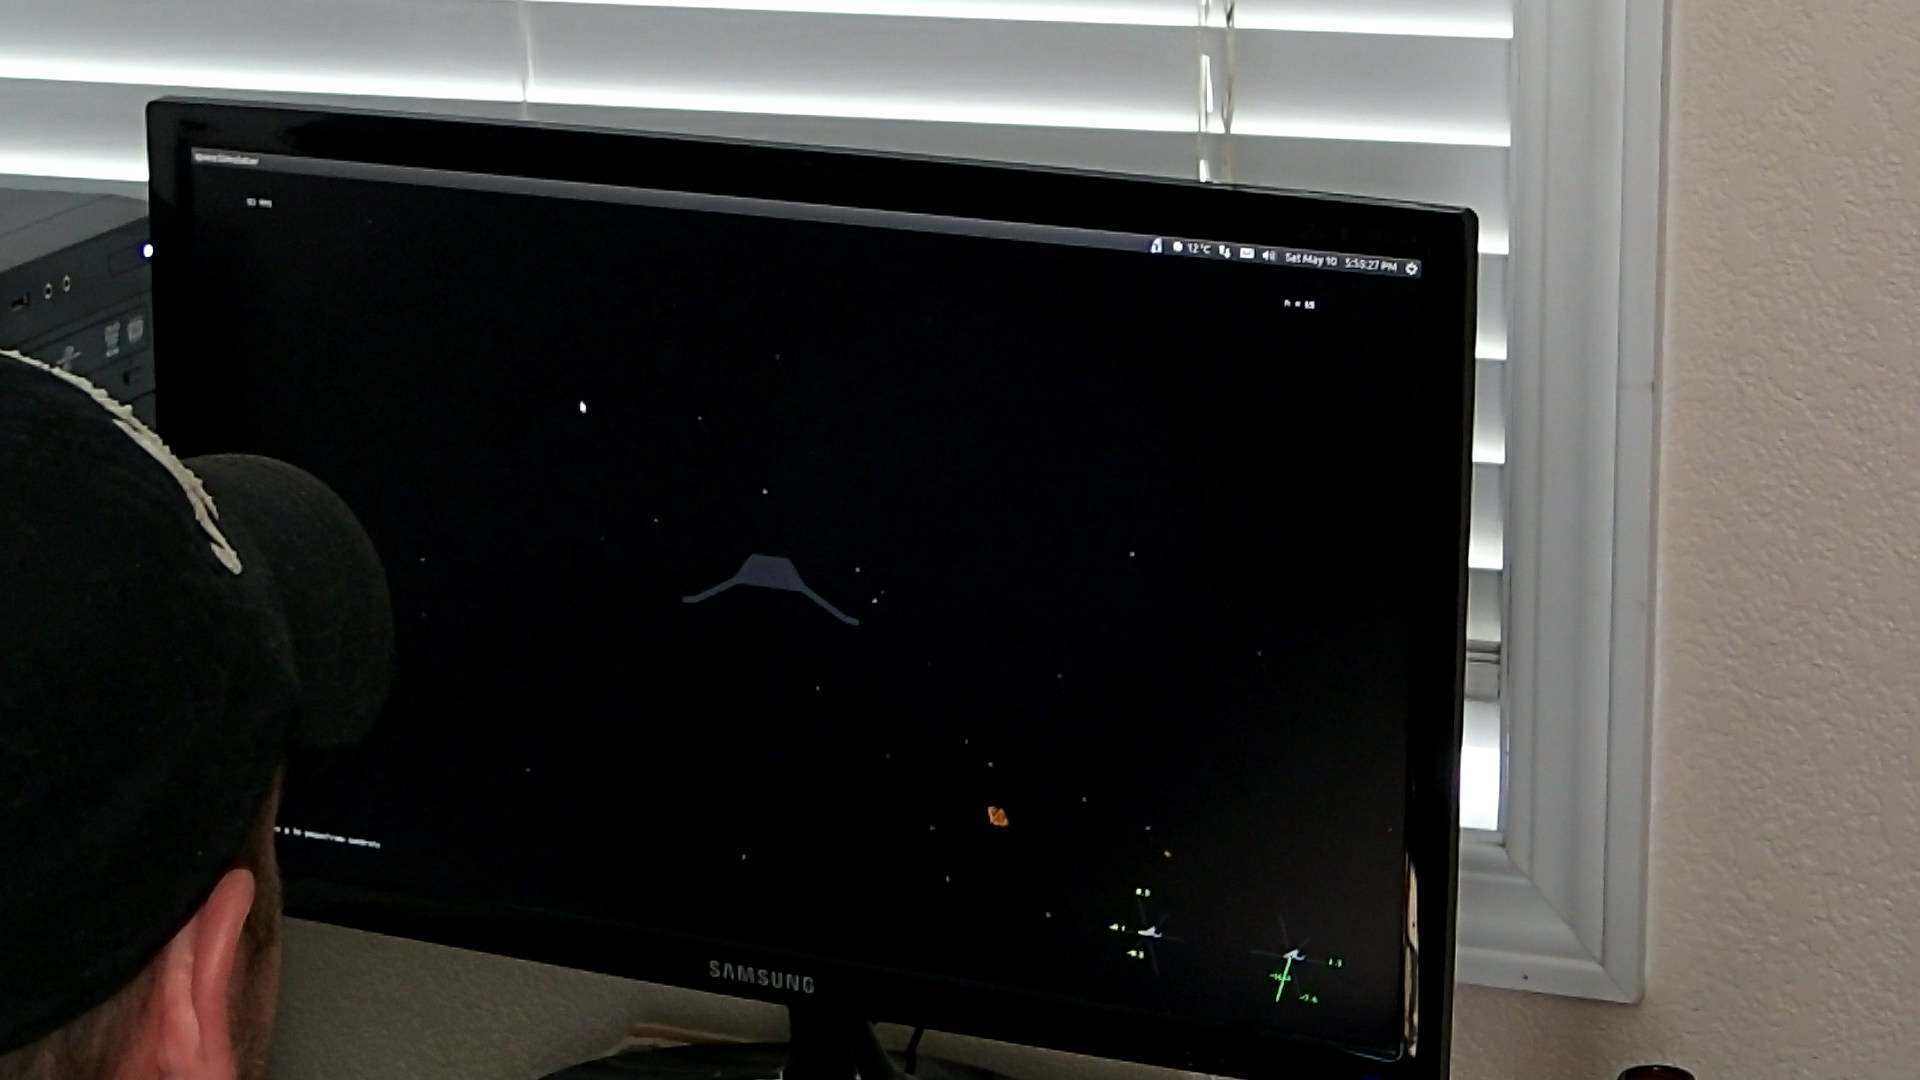
\includegraphics[width=1.0\textwidth]{images/ss5.jpg}
  \caption{Again, attempting to catch up with the planet.  Frustrations mount as questions asked could not be answered.}
\end{figure}

\subsection{Problem areas and possible solutions}

We have highlighted major problem areas and identified solutions below.

\begin{itemize}

  \item \emph{Several players mixed up the ``yaw'' and ``strafe'' controls.}
        
        \textbf{Possible Solution : } \parbox[t]{5in}{Swap the keys for ``yaw'' and ``strafe'' or provide a tutorial describing the controls.}
				
  \item \emph{The controls appeared too sensitive. Often, players would press keys and get more feedback than they expected.}
        
        \textbf{Possible Solution : } \parbox[t]{5in}{Slow down the time-step to make corrections easier.  The time-step was reduced for the last two simulations with improved results; the players could more easily control the craft.}
				
  \item \emph{Nearly all players entered uncontrollable spins and expressed a desire to have a button that resets the ship to the start position.}
        
        \textbf{Possible Solution : } \parbox[t]{5in}{Have a ``tutorial'' mode that has a button that stops all movement.}

  \item \emph{Several players frequently paused to review controls.}
        
        \textbf{Possible Solution : } \parbox[t]{5in}{List all controls at all times, at least in the ``tutorial'' mode.}
				
	\item \emph{Several players expressed frustration with the inverted controls.}
        
        \textbf{Possible Solution : } \parbox[t]{5in}{Add a key to toggle inverted controls on/off.}	

	\item \emph{The learning curve was very steep. Several players seemed to take a while to understand the controls and vectors.}
        
        \textbf{Possible Solution : } \parbox[t]{5in}{An extensive tutorial is most likely required.}	

	\item \emph{Ascend and descend controls were not often used.  Players also reported that the \texttt{page up} and \texttt{page down} controls were not intuitive.}
        
        \textbf{Possible Solution : } \parbox[t]{5in}{Change the controls to a joystick or allow the user to define their own control mapping.}

	\item \emph{The ``yaw'' controls were frequently forgotten.}
        
        \textbf{Possible Solution : } \parbox[t]{5in}{A tutorial which requires the use of ``yaw'' to complete.}

	\item \emph{Difficult to determine when to apply a translational or rotational force; participants confused which control they needed to use to stop rotating or translating.}
        
        \textbf{Possible Solution : } \parbox[t]{5in}{During a severe spin, highlight the rotational controls.  Experience playing the game eliminates this problem.}

	\item \emph{Velocity vectors were difficult to interpret.}
        
        \textbf{Possible Solution : } \parbox[t]{5in}{show the vector on the ship itself, instead of separate.  We could also render the vector differently to help show precisely where it was pointing.}

\end{itemize}

\end{document}


